\documentclass[12pt,fleqn]{article}\usepackage{../../common}
\begin{document}
Tensorflow ile Regresyon, YSA

Toptan basit lineer regresyon hesabını Tensorflow [5] ile nasıl yaparız?
Regresyonu California emlak veri seti üzerinde işleteceğiz, bu veride bölge
bazlı olarak ev sahiplerinin ortalama yaşı, geliri, gibi değişkenler ile hedef
değişkeni olan ev fiyatı kayıtlı. Hedef ve kaynak değişkenler arasındaki lineer
ilişki lineer regresyon ile hesaplanabilir, tanıdık formül,

$\hat{\theta} = (X^TX )^{-1} X^T y $

Veriye bir yanlılık (sadece 1 değeri içeren yeni bir kolon) ekleyip üstteki
hesabı yapalım.

\begin{minted}[fontsize=\footnotesize]{python}
import tensorflow as tf
from sklearn.datasets import fetch_california_housing
from sklearn.preprocessing import StandardScaler

def reset_graph(seed=42):
    tf.reset_default_graph()
    tf.set_random_seed(seed)
    np.random.seed(seed)

housing = fetch_california_housing(data_home="/home/burak/Downloads/scikit-data")
print housing['data'].shape
print housing['target'][:5]

m, n = housing.data.shape

housing_data_plus_bias = np.c_[np.ones((m, 1)), housing.data]
X = tf.constant(housing_data_plus_bias, dtype=tf.float32, name="X")
y = tf.constant(housing.target.reshape(-1, 1), dtype=tf.float32, name="y")
XT = tf.transpose(X)
theta = tf.matmul(tf.matmul(tf.matrix_inverse(tf.matmul(XT, X)), XT), y)

with tf.Session() as sess:
    theta_value = theta.eval()
print 'theta'
print theta_value
\end{minted}

\begin{verbatim}
(20640, 8)
[ 4.526  3.585  3.521  3.413  3.422]
theta
[[ -3.68059006e+01]
 [  4.36796039e-01]
 [  9.45724174e-03]
 [ -1.07348330e-01]
 [  6.44418657e-01]
 [ -3.95741154e-06]
 [ -3.78908939e-03]
 [ -4.20193195e-01]
 [ -4.33070064e-01]]
\end{verbatim}

TF'in matris çarpımı için \verb!matmul!, tersini alma için
\verb!matrix_inverse! çağrılarını görüyoruz. Üstteki kodu olduğu gibi alıp
pek çok işlemci üzerinde direk paralel şekilde işletebiliriz, aynı işi pür
numpy bazlı kodla yapmak daha külfetli olurdu.

Gradyan İnişi

Klasik toptan usül ile hesabı gördük. Peki gradyan inişi ile lineer
regresyon nasıl yaparız? Burada iki yaklaşımı göstereceğiz, biri daha zor,
diğeri daha kolay. Zor olan matematiksel olarak elle kendimizin gradyan
türevini alması, daha kolay olanı türevi TF içindeki otomatik türev alma
mekanizmasını kullanarak o işi de TF'e yaptırmak.

Veriyi hazırlayalım ve çiziti oluşturalım; başlangıç $\theta$ değeri
rasgele atansın, $X,y$ değerleri verinin kendisi olacak, tahmin ve hata
için fonksiyonlar olsun.

\begin{minted}[fontsize=\footnotesize]{python}
scaler = StandardScaler()
scaled_housing_data = scaler.fit_transform(housing.data)
scaled_housing_data_plus_bias = np.c_[np.ones((m, 1)), scaled_housing_data]

reset_graph()

X = tf.constant(scaled_housing_data_plus_bias, dtype=tf.float32, name="X")
y = tf.constant(housing.target.reshape(-1, 1), dtype=tf.float32, name="y")
theta = tf.Variable(tf.random_uniform([n + 1, 1], -1.0, 1.0, seed=42), name="theta")
y_pred = tf.matmul(X, theta, name="predictions")
error = y_pred - y
mse = tf.reduce_mean(tf.square(error), name="mse")
\end{minted}

Elle türevi alınmış gradyan nedir? [1, sf. 261]'e göre formül

$$ 
\nabla_\theta MSE(\theta) = \frac{2}{m} X^T (X \cdot \theta - y)
$$  

ve gradyan güncellemesi

$$ 
\theta^{t+1} = \theta - \eta \nabla_\theta MSE(\theta)
$$

Alttaki TF kodu bir döngü içinde gradyan güncellemesi yapacak ve hata
karelerinin ortalaması (mean square error -MSE-) hesaplayıp ekrana
basacak. MSE'in gittikçe aşağı inmesi lazım, çünkü gradyanın tersi yönünde
hatayı azaltacak şekilde hareket ediyoruz. 

\begin{minted}[fontsize=\footnotesize]{python}
n_epochs = 1000
learning_rate = 0.01

gradients = 2/np.float(m) * tf.matmul(tf.transpose(X), error)
training_op = tf.assign(theta, theta-(learning_rate*gradients))

init = tf.global_variables_initializer()

with tf.Session() as sess:
    sess.run(init)
    for epoch in range(n_epochs):
        if epoch % 100 == 0: print("Epoch", epoch, "MSE =", mse.eval())
	sess.run(training_op)    
    best_theta = theta.eval()
    
print 'theta'
print best_theta
\end{minted}

\begin{verbatim}
('Epoch', 0, 'MSE =', 9.1615429)
('Epoch', 100, 'MSE =', 0.71450073)
('Epoch', 200, 'MSE =', 0.56670469)
('Epoch', 300, 'MSE =', 0.55557162)
('Epoch', 400, 'MSE =', 0.54881161)
('Epoch', 500, 'MSE =', 0.54363626)
('Epoch', 600, 'MSE =', 0.53962916)
('Epoch', 700, 'MSE =', 0.53650916)
('Epoch', 800, 'MSE =', 0.53406781)
('Epoch', 900, 'MSE =', 0.53214705)
theta
[[ 2.06855249]
 [ 0.88740271]
 [ 0.14401658]
 [-0.34770882]
 [ 0.36178368]
 [ 0.00393812]
 [-0.04269557]
 [-0.66145277]
 [-0.63752776]]
\end{verbatim}

Otomatik Türev ile Gradyan

Sembolik türev yerine TF içindeki \verb!autodiff! paketine türevi aldıralım
ve gradyan inişini böyle yapalım,

\begin{minted}[fontsize=\footnotesize]{python}
gradients = tf.gradients(mse, [theta])[0] # otomatik turev

training_op = tf.assign(theta, theta-(learning_rate*gradients))

init = tf.global_variables_initializer()

with tf.Session() as sess:
    sess.run(init)
    for epoch in range(n_epochs):
        if epoch % 100 == 0: print("Epoch", epoch, "MSE =", mse.eval())
	sess.run(training_op)
    
    best_theta = theta.eval()
    
print best_theta
\end{minted}

\begin{verbatim}
('Epoch', 0, 'MSE =', 9.1615429)
('Epoch', 100, 'MSE =', 0.71450061)
('Epoch', 200, 'MSE =', 0.56670463)
('Epoch', 300, 'MSE =', 0.55557162)
('Epoch', 400, 'MSE =', 0.54881167)
('Epoch', 500, 'MSE =', 0.5436362)
('Epoch', 600, 'MSE =', 0.53962916)
('Epoch', 700, 'MSE =', 0.53650916)
('Epoch', 800, 'MSE =', 0.53406781)
('Epoch', 900, 'MSE =', 0.53214717)
[[ 2.06855249]
 [ 0.88740271]
 [ 0.14401658]
 [-0.34770882]
 [ 0.36178368]
 [ 0.00393811]
 [-0.04269556]
 [-0.66145277]
 [-0.6375277 ]]
\end{verbatim}

Aynı sonuca eriştik. 

Daha da basitleştirebiliriz, üstteki kodda \verb!assign! ile gradyan inişi
için gereken çıkartma işlemi elle yapıldı. TF paketi içinde bu çıkartmayı
yapacak optimizasyon rutinleri de var, mesela
\verb!GradientDescentOptimizer!.

\begin{minted}[fontsize=\footnotesize]{python}
optimizer = tf.train.GradientDescentOptimizer(learning_rate=learning_rate)
training_op = optimizer.minimize(mse)

init = tf.global_variables_initializer()

with tf.Session() as sess:
    sess.run(init)
    for epoch in range(n_epochs):
        if epoch % 100 == 0: print("Epoch", epoch, "MSE =", mse.eval())
        sess.run(training_op)    
    best_theta = theta.eval()

print('theta')
print(best_theta)
\end{minted}

\begin{verbatim}
('Epoch', 0, 'MSE =', 9.1615429)
('Epoch', 100, 'MSE =', 0.71450061)
('Epoch', 200, 'MSE =', 0.56670463)
('Epoch', 300, 'MSE =', 0.55557162)
('Epoch', 400, 'MSE =', 0.54881167)
('Epoch', 500, 'MSE =', 0.5436362)
('Epoch', 600, 'MSE =', 0.53962916)
('Epoch', 700, 'MSE =', 0.53650916)
('Epoch', 800, 'MSE =', 0.53406781)
('Epoch', 900, 'MSE =', 0.53214717)
theta
[[ 2.06855249]
 [ 0.88740271]
 [ 0.14401658]
 [-0.34770882]
 [ 0.36178368]
 [ 0.00393811]
 [-0.04269556]
 [-0.66145277]
 [-0.6375277 ]]
\end{verbatim}

Görüldüğü gibi matris işlemi içeren her türlü hesap TF ile kodlanabilir, bu
yapıldığında kodlar rahat bir şekilde paralelize edilebilir. Yapay
öğrenimde ne kadar çok lineer cebir kullanımı olduğunu biliyoruz, ayrıca
türev almak otomatikleştirildiği için akla gelebilecek her türlü lineer
cebir, optimizasyon işlemi TF üzerinden kodlanabilir.

TensorFlow ile Çok Katmanlı Yapay Sinir Ağları (Neural Network -NN-)

Şimdi çok katmanlı NN ile regresyon yapma örneği görelim. Bir NN bildiğimiz
gibi evrensel yaklaşıklayıcı, yeterli veri var ise her türlü fonksiyonu
yaklaşık olarak temsil edebilir, öğrenebilir. Düz lineer regresyon ile
yaptığımız da bir bakıma budur, bilinmeyen bir fonksiyonu veriden öğrenmeye
uğraşırız, fakat nihai fonksiyon lineer olmalı. NN ile lineer, gayrı-lineer
her türlü fonksiyon temsil edilebilir.

Her katmanda girdi ağırlıklar ile çarpılacak, bir yanlılık (bias)
eklenecek, ve sonuç bir aktivasyon fonksiyonuna verilecek (altta kullanılan
ReLu), buradan çıkan sonuç bir sonraki katmana aktarılacak. Aktivasyon
lazım çünkü aktivasyon olmasa, her katman sadece ağırlıklarla çarpılan
sonucu bir sonraki katmana verse, tüm NN'in işlemi ardı ardına matrislerin
çarpımı olarak ta görülebilirdi, ama bu bir lineer işlem olurdu, o zaman NN
gayri-lineerligi modelleyemezdi. Diğer yandan lineer regresyon bir bakıma
tek katmanlı ve aktivasyonu olmayan bir NN gibi görülebilir.

Örnek için kullanılan veri seti Low Birth Weight [2] verisi, bu veride
yeni doğan çocukların annenin tıbbi verileri ile çocuğun doğduğundaki
ağırlığı kaydedilmiş, ve bu hedef değişkeni ile diğerleri arasındaki
ilişkiyi öğrenmek istiyoruz. Veriyi okuyup normalize edelim,

\begin{minted}[fontsize=\footnotesize]{python}
from tensorflow.python.framework import ops
import pandas as pd
import tensorflow as tf

cols_of_interest = ['AGE', 'LWT', 'RACE', 'SMOKE', 'PTL', 'HT', 'UI', 'FTV']
df = pd.read_csv('lowbwt.dat',sep='\s*',engine='python')
x_vals = np.array(df[cols_of_interest])
y_vals = np.array(df['BWT'])

ops.reset_default_graph()
tf.set_random_seed(3)
np.random.seed(3)

sess = tf.Session()

tmp = np.random.choice(range(len(x_vals)), size=len(x_vals), replace=False)
first = int(len(x_vals)*0.80)
train_indices = tmp[:first]
test_indices = tmp[first:]

x_vals_train = x_vals[train_indices]
x_vals_test = x_vals[test_indices]
y_vals_train = y_vals[train_indices]
y_vals_test = y_vals[test_indices]

def normalize_cols(m):
    col_max = m.max(axis=0)
    col_min = m.min(axis=0)
    return (m-col_min) / (col_max - col_min)
    
x_vals_train = np.nan_to_num(normalize_cols(x_vals_train))
x_vals_test = np.nan_to_num(normalize_cols(x_vals_test))
\end{minted}

NN katmanlarını hazırlayalım [3], üç katman olacak, katmanlarda sırasıyla
25, 10 ve 3 tane nöron olacak. Kayıp (loss) fonksiyonu L1 (mutlak değer)
üzerinden hesaplanıyor. Optimize edici olarak TF'in
\verb!AdamOptimizer!'ini kullanacağız.

\begin{minted}[fontsize=\footnotesize]{python}
def init_weight(shape, st_dev):
    weight = tf.Variable(tf.random_normal(shape, stddev=st_dev))
    return(weight)
    
def init_bias(shape, st_dev):
    bias = tf.Variable(tf.random_normal(shape, stddev=st_dev))
    return(bias)
    
x_data = tf.placeholder(shape=[None, 8], dtype=tf.float32)
y_target = tf.placeholder(shape=[None, 1], dtype=tf.float32)

def fully_connected(input_layer, weights, biases):
    layer = tf.add(tf.matmul(input_layer, weights), biases)
    return(tf.nn.relu(layer))

weight_1 = init_weight(shape=[8, 25], st_dev=10.0)
bias_1 = init_bias(shape=[25], st_dev=10.0)
layer_1 = fully_connected(x_data, weight_1, bias_1)

weight_2 = init_weight(shape=[25, 10], st_dev=10.0)
bias_2 = init_bias(shape=[10], st_dev=10.0)
layer_2 = fully_connected(layer_1, weight_2, bias_2)

weight_3 = init_weight(shape=[10, 3], st_dev=10.0)
bias_3 = init_bias(shape=[3], st_dev=10.0)
layer_3 = fully_connected(layer_2, weight_3, bias_3)

weight_4 = init_weight(shape=[3, 1], st_dev=10.0)
bias_4 = init_bias(shape=[1], st_dev=10.0)
final_output = fully_connected(layer_3, weight_4, bias_4)

loss = tf.reduce_mean(tf.abs(y_target - final_output))

my_opt = tf.train.AdamOptimizer(0.02)
train_step = my_opt.minimize(loss)

init = tf.initialize_all_variables()
sess.run(init)
\end{minted}

NN ağ çizit yapısı kuruldu, hatta ağırlıkların değerleri bile var. Tabii
başta bu değerler rasgele değerler, yani istediğimiz nihai değerler
değiller. Fakat üsttekinin geçerli bir NN olduğunu ispatlamak için
dışarıdan bir test verisi versek bize bir hesap yapacağını göreceğiz. Bunun
için yer tutuculara tek bir veri noktası verelim, ve sonuç düğümünün
hesaplanmasını isteyelim,

\begin{minted}[fontsize=\footnotesize]{python}
x = np.array([20.,181.,1.,1.,0.,0.,1.,0.]) # uyduruk veri
x = np.reshape(x, (1,8))
print sess.run(final_output,feed_dict={x_data: x})
\end{minted}

\begin{verbatim}
[[ 8723006.]]
\end{verbatim}

Bu sayı çok büyük, problem açısından tabii ki anlamsız, NN'i eğitim
verisiyle eğittikçe NN ağırlıkları gerçek hallerine yaklaşacaklar, o zaman
üstteki gibi bir veri noktası için daha iyi bir sonuç alabileceğiz, fakat
bir hesabın yapılabildiğini görüyoruz.

Şimdi veriyi 80/20 oranında eğitim / doğrulama olarak ayıralım, ve eğitim
veri seti üzerinde eğitim yapalım. Eğitim verisinden \verb!batch_size!
büyüklüğünde mini toptan parçalar (minibatch) örnekleyelim, ve her eğitim
döngüsünde optimize ediciye bu parçaları verelim.

\begin{minted}[fontsize=\footnotesize]{python}
loss_vec = []; test_loss = []

batch_size = 200

for i in range(200):
    rand_index = np.random.choice(len(x_vals_train), size=batch_size)
    rand_x = x_vals_train[rand_index]
    rand_y = np.transpose([y_vals_train[rand_index]])
    sess.run(train_step, feed_dict={x_data: rand_x, y_target: rand_y})

    temp_loss = sess.run(loss, feed_dict={x_data: rand_x, y_target: rand_y})
    loss_vec.append(temp_loss)

    d = {x_data: x_vals_test, y_target: np.transpose([y_vals_test])}
    test_temp_loss = sess.run(loss, feed_dict=d)
    test_loss.append(test_temp_loss)
    if (i+1)%25==0:
        print('Epoch: ' + str(i+1) + '. Kayip = ' + str(temp_loss))

# Plot loss over time
plt.plot(loss_vec, 'k-', label=u'Eğitim Kaybı')
plt.plot(test_loss, 'r--', label=u'Test Kaybı')
plt.title(u'Her Epoch İçinde Kayıp')
plt.xlabel('Epoch')
plt.ylabel(u'Kayıp')
plt.legend(loc="upper right")
plt.savefig('tf_03.png')
\end{minted}

\begin{verbatim}
Epoch: 25. Kayip = 16744.3
Epoch: 50. Kayip = 8367.32
Epoch: 75. Kayip = 4687.56
Epoch: 100. Kayip = 1767.07
Epoch: 125. Kayip = 1297.27
Epoch: 150. Kayip = 852.689
Epoch: 175. Kayip = 705.81
Epoch: 200. Kayip = 728.779
\end{verbatim}

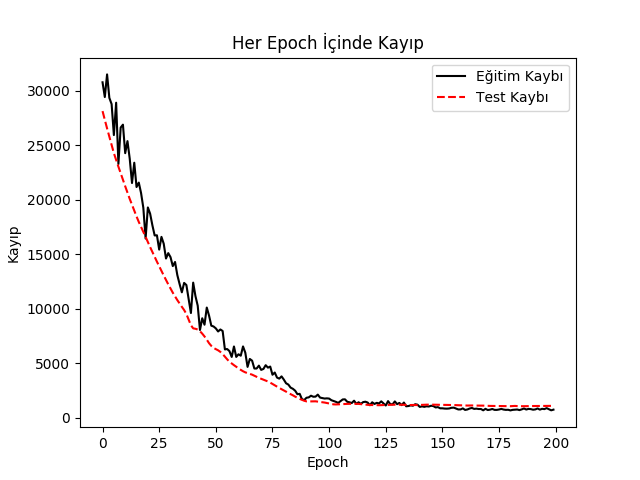
\includegraphics[width=30em]{tf_03.png}

Görüldüğü gibi eğitim ve test kaybı birbirine yakın ki bu iyiye işaret,
model iyi öğreniyor, eksik uyum, aşırı uyum durumları yok demektir, ve
nihai kayıp her iki tarafta da 0.7 kg civarı.

Not: Girdi verisinde yaklaşık 200 satır veri olduğuna dikkat, şu
sorulabilir, eğitim sırasında 200 kere dönüyoruz, her döngüde 200 civarı
toptan parça kullanıyoruz, bu nasıl oluyor? Ufak parçaların içeriğini {\em
 örnekliyoruz}, o zaman döngü sayısı, parça sayısına bakarsak bir anlamda
veriyi örnekleyerek çoğaltmış (upsample) oluyoruz. Bu NN eğitiminde sürekli
ortaya çıkan bir kavram, aklımızda olsun. 

İki Kategori Sınıflaması

Peki istatistikte lojistik regresyon ile yaptığımız iki kategori arasında
sınıflamayı çok katmanlı NN ile nasıl yaparız? Mesela bebeğin 2.5 kg
altında doğup doğmaması diyelim, bu bir riskli durum, ve iki farklı sınıf
olarak görülebilecek bu hedef değişkeni için 0/1 tarzında bir eğitim yapmak
istiyoruz. İlk akla gelebilecek çözüm bir önceki NN'i alıp oradan gelecek
tahminleri eşik değeri 2.5 üstünde mi altında mı diye ek bir filtrelemeden
geçirmek, yani regresyon sonucunu 0/1 tahminine çevirmek.  Bu yaklaşım
yüzde 55 civarı başarı veriyor.

Daha iyisi, daha farklı bir NN'i özellikle 0/1 hedefi için eğitmek.

\begin{minted}[fontsize=\footnotesize]{python}
from tensorflow.python.framework import ops
import pandas as pd
import tensorflow as tf

cols_of_interest = ['AGE', 'LWT', 'RACE', 'SMOKE', 'PTL', 'HT', 'UI', 'FTV']
df = pd.read_csv('lowbwt.dat',sep='\s*',engine='python')
x_vals = np.array(df[cols_of_interest])
y_vals = np.array(df['LOW'])

ops.reset_default_graph()
tf.set_random_seed(1)
np.random.seed(1)
sess = tf.Session()

tmp = np.random.choice(range(len(x_vals)), size=len(x_vals), replace=False)
first = int(len(x_vals)*0.80)
train_indices = tmp[:first]
test_indices = tmp[first:]

x_vals_train = x_vals[train_indices]
x_vals_test = x_vals[test_indices]
y_vals_train = y_vals[train_indices]
y_vals_test = y_vals[test_indices]

def normalize_cols(m):
    col_max = m.max(axis=0)
    col_min = m.min(axis=0)
    return (m-col_min) / (col_max - col_min)
    
x_vals_train = np.nan_to_num(normalize_cols(x_vals_train))
x_vals_test = np.nan_to_num(normalize_cols(x_vals_test))

batch_size = 50

x_data = tf.placeholder(shape=[None, 8], dtype=tf.float32)
y_target = tf.placeholder(shape=[None, 1], dtype=tf.float32)

def init_variable(shape):
    return(tf.Variable(tf.random_normal(shape=shape)))

def logistic(input_layer, multiplication_weight, bias_weight, activation = True):
    linear_layer = tf.add(tf.matmul(input_layer, multiplication_weight), bias_weight)
    if activation:
        return(tf.nn.sigmoid(linear_layer))
    else:
        return(linear_layer)
\end{minted}

Üstteki \verb!logistic! çağrısı ağırlıklarla çarpım sonucunu bir sigmoid
fonksiyonundan geçiriyor. Yeni NN'imiz 20, 20, 10 nöron içeren bu yeni
stili kullanacak.

\begin{minted}[fontsize=\footnotesize]{python}
A1 = init_variable(shape=[8,20])
b1 = init_variable(shape=[20])
logistic_layer1 = logistic(x_data, A1, b1)

A2 = init_variable(shape=[20,10])
b2 = init_variable(shape=[10])
logistic_layer2 = logistic(logistic_layer1, A2, b2)

A3 = init_variable(shape=[10,1])
b3 = init_variable(shape=[1])
final_output = logistic(logistic_layer2, A3, b3, activation=False)

tmp = tf.nn.sigmoid_cross_entropy_with_logits(logits=final_output, labels=y_target)
loss = tf.reduce_mean(tmp)
     
my_opt = tf.train.AdamOptimizer(learning_rate = 0.002)
train_step = my_opt.minimize(loss)

init = tf.global_variables_initializer()
sess.run(init)

prediction = tf.round(tf.nn.sigmoid(final_output))
predictions_correct = tf.cast(tf.equal(prediction, y_target), tf.float32)
accuracy = tf.reduce_mean(predictions_correct)
\end{minted}

\begin{minted}[fontsize=\footnotesize]{python}
loss_vec = []; train_acc = []; test_acc = []

for i in range(1500):
    rand_index = np.random.choice(len(x_vals_train), size=batch_size)
    rand_x = x_vals_train[rand_index]
    rand_y = np.transpose([y_vals_train[rand_index]])

    sess.run(train_step, feed_dict={x_data: rand_x, y_target: rand_y})
    temp_loss = sess.run(loss, feed_dict={x_data: rand_x, y_target: rand_y})
    loss_vec.append(temp_loss)

    d1 = {x_data: x_vals_train, y_target: np.transpose([y_vals_train])}
    temp_acc_train = sess.run(accuracy, feed_dict=d1)
    train_acc.append(temp_acc_train)

    d2 = {x_data: x_vals_test, y_target: np.transpose([y_vals_test])}
    temp_acc_test = sess.run(accuracy, feed_dict=d2)
    test_acc.append(temp_acc_test)
    if (i+1)%150==0: print('Loss = ' + str(temp_loss))

plt.plot(loss_vec, 'k-')
plt.title(u"Her Epoch İçin Çapraz Entropi Kaybı")
plt.xlabel(u"Epoch")
plt.ylabel(u"Çapraz Entropi Kaybı")
plt.ylim(0.0,2.0)
plt.savefig('tf_04.png')        

plt.figure()
plt.plot(train_acc, 'k-', label=u"Eğitim Seti Doğrulugu")
plt.plot(test_acc, 'r--', label=u"Test Set Doğrulugu")
plt.title(u"Eğitim ve Test Doğruluğu")
plt.xlabel("Epoch")
plt.ylabel(u"Doğruluk")
plt.ylim(0.0,0.8)
plt.legend(loc='lower right')
plt.savefig('tf_05.png')        
\end{minted}

\begin{verbatim}
Loss = 0.615425
Loss = 0.593725
Loss = 0.575125
Loss = 0.664008
Loss = 0.667132
Loss = 0.617393
Loss = 0.504238
Loss = 0.447125
Loss = 0.530287
Loss = 0.528585
\end{verbatim}

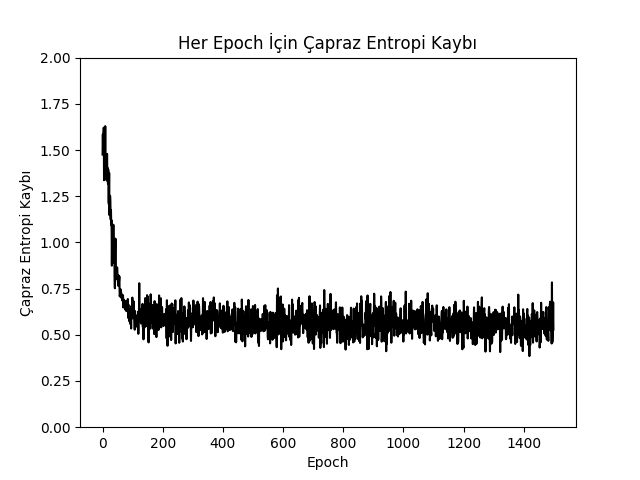
\includegraphics[width=30em]{tf_04.png}

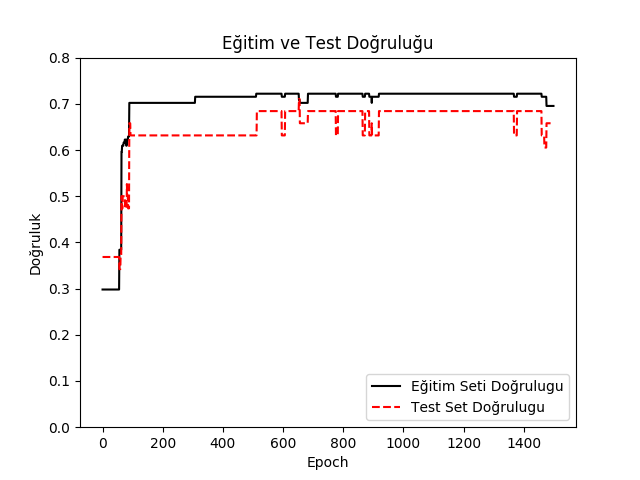
\includegraphics[width=30em]{tf_05.png}

Çoklu Kategori Hedefi

Çiçeklerin ölçümleri ve çiçek çeşitlerini içeren ünlü IRIS veri setinde 4
boyutlu sayısal veri ile 3 çiçek çeşidi arasında softmax ile seçim yapacak
bir kodu görelim. Bu kodda tamamen tamamen bağlanmış katman
(fully-connected layer) hesabını elle değil, TF çağrısı
\verb!tf.contrib.layers.fully_connected! ile yapıyoruz. 

İlk önce sadece tek tamamen bağlanmış katman içeren bir kod görelim,

\begin{minted}[fontsize=\footnotesize]{python}
import pandas as pd
import tensorflow as tf
from sklearn.model_selection import train_test_split
from sklearn import preprocessing

np.random.seed(0)
tf.set_random_seed(0)

cols = ["sepal_length", "sepal_width", "petal_length", "petal_width", "iris_class"]
data = pd.read_csv("iris.data", sep=",",names=cols)
data = data.sample(frac=1,random_state=0).reset_index(drop=True)
all_x = data[["sepal_length", "sepal_width", "petal_length", "petal_width"]]
min_max_scaler = preprocessing.MinMaxScaler()
all_x = min_max_scaler.fit_transform(all_x)
all_y = pd.get_dummies(data.iris_class)
train_x, test_x, train_y, test_y = train_test_split(all_x, all_y, test_size=0.20)

print(train_x.shape)
print(train_y.shape)
print(test_x.shape)
print(test_y.shape)

tf.reset_default_graph()

learning_rate = 0.01

x = tf.placeholder(tf.float32, [None, np.shape(train_x)[1]], name="x")
y = tf.placeholder(tf.float32, [None, np.shape(train_y)[1]], name="y")

prediction = tf.contrib.layers.fully_connected(inputs=x,
                                               num_outputs=np.shape(train_y)[1], 
                                               activation_fn=tf.nn.softmax)

cost = tf.losses.softmax_cross_entropy(onehot_labels=y,logits=prediction)

correct_prediction = tf.equal(tf.argmax(prediction,1),tf.argmax(y, 1))

accuracy = tf.reduce_mean(tf.cast(correct_prediction,tf.float32))

optimizer = tf.train.AdagradOptimizer(learning_rate).minimize(cost)

sess = tf.InteractiveSession()

init = tf.global_variables_initializer()

sess.run(init)

training_epochs = 3000
for epoch in range(training_epochs):
    sess.run([optimizer, cost], feed_dict={x: train_x, y: train_y})

print("Dogruluk:", accuracy.eval({x: test_x, y: test_y}))    
\end{minted}

\begin{verbatim}
(120, 4)
(120, 3)
(30, 4)
(30, 3)
('Dogruluk:', 0.76666665)
\end{verbatim}

Şimdi sırasıyla 10,20,10 olacak şekilde üç katmanlı bir YSA ile sınıflama
yapalım,

\begin{minted}[fontsize=\footnotesize]{python}
tf.reset_default_graph()

learning_rate = 0.01

x = tf.placeholder(tf.float32, [None, np.shape(train_x)[1]], name="x")
y = tf.placeholder(tf.float32, [None, np.shape(train_y)[1]], name="y")

h1 = 10 # 1. gizli (hidden) katman
h2 = 20 # 2. gizli katman
h3 = 10 # 3. gizli katman

k1 = tf.contrib.layers.fully_connected(inputs=x,
                                       num_outputs=h1, 
                                       activation_fn=tf.nn.relu)

k2 = tf.contrib.layers.fully_connected(inputs=k1,
                                       num_outputs=h2, 
                                       activation_fn=tf.nn.relu)

k3 = tf.contrib.layers.fully_connected(inputs=k2,
                                       num_outputs=h3, 
                                       activation_fn=tf.nn.relu)

prediction = tf.contrib.layers.fully_connected(inputs=k3,
                                               num_outputs=np.shape(train_y)[1], 
                                               activation_fn=tf.nn.softmax)

cost = tf.losses.softmax_cross_entropy(onehot_labels=y,logits=prediction)

correct_prediction = tf.equal(tf.argmax(prediction,1),tf.argmax(y, 1))

accuracy = tf.reduce_mean(tf.cast(correct_prediction,tf.float32))

optimizer = tf.train.AdagradOptimizer(learning_rate).minimize(cost)

sess = tf.InteractiveSession()

init = tf.global_variables_initializer()

sess.run(init)

training_epochs = 3000
for i in range(training_epochs):
    sess.run([optimizer, cost], feed_dict={x: train_x, y: train_y})

print("Dogruluk:", accuracy.eval({x: test_x, y: test_y}))    
\end{minted}

\begin{verbatim}
('Dogruluk:', 0.96666664)
\end{verbatim}

Notlar

Vektorler, gradyanlar hakkinda birkac cabuk not,

\begin{minted}[fontsize=\footnotesize]{python}
import tensorflow as tf

# y + 2x = 2x + x
x = tf.constant(0.)
y = 2 * x
g1 = tf.gradients(x + y, [x, y])

xvec = tf.Variable([[1.], [2.],[3.]]) 
yvec = tf.Variable([[3.], [4.],[5.]]) 
xvec = xvec + np.array([[1, 1, 1]]).T
zvec = tf.matmul(tf.transpose(xvec),yvec)
g2 = tf.gradients(zvec, xvec)

with tf.Session() as sess:
    sess.run(tf.global_variables_initializer())
    print (sess.run(g1))
    print (sess.run(xvec))
    print (sess.run(yvec))
    print (sess.run(zvec))
    print (sess.run(g2))
\end{minted}

\begin{verbatim}
[3.0, 1.0]
[[2.]
 [3.]
 [4.]]
[[3.]
 [4.]
 [5.]]
[[38.]]
[array([[3.],
       [4.],
       [5.]], dtype=float32)]
\end{verbatim}

Kaynaklar 

[1] Géron, {\em Hands-On Machine Learning with Scikit-Learn and TensorFlow}

[2] Heidelberg U., {\em Risk Factors Associated with Low Infant Birth Weight}, \url{http://www.statlab.uni-heidelberg.de/data/linmod/birthweight.html}

[3] McClure, {\em TensorFlow Machine Learning Cookbook}

[4] Bayramli, Bilgisayar Bilim, {\em Otomatik Türev Almak}

[5] Bayramli, Tensorflow, 

\end{document}
